\documentclass[border=10pt]{standalone}
\usepackage{tikz}
\usetikzlibrary{automata, positioning, arrows.meta, calc}

\begin{document}
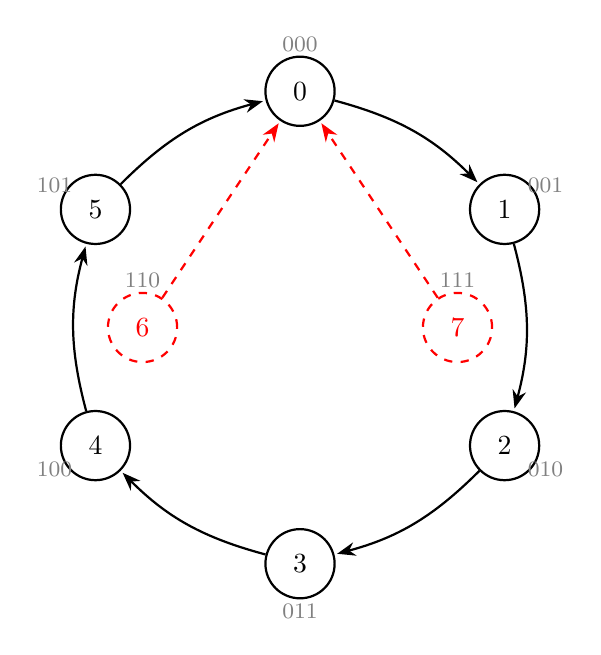
\begin{tikzpicture}[
    ->, >=Stealth, 
    shorten >=1pt, 
    auto, 
    node distance=2.5cm, 
    thick
]

    % Define radius for the main cycle
    \def\radius{3.0cm}
    
    % Valid states 0-5 in a circle
    \foreach \i in {0,...,5} {
        % 360/6 = 60 degrees. Start at 90.
        \pgfmathsetmacro{\angle}{90 - \i * 60}
        \node[state] (s\i) at (\angle:\radius) {\i};
    }
    
    % Invalid states 6 and 7 inside
    \node[state, dashed, color=red] (s6) at (-2,0) {\textcolor{red}{6}};
    \node[state, dashed, color=red] (s7) at (2,0) {\textcolor{red}{7}};
    
    % Normal Transitions
    \path (s0) edge [bend left=15] (s1)
          (s1) edge [bend left=15] (s2)
          (s2) edge [bend left=15] (s3)
          (s3) edge [bend left=15] (s4)
          (s4) edge [bend left=15] (s5)
          (s5) edge [bend left=15] (s0);
          
    % Self-correction Transitions
    \path[dashed, color=red] (s6) edge  (s0);
    \path[dashed, color=red] (s7) edge  (s0);

    % Binary Labels (optional, but helpful)
    \foreach \i/\bin in {0/000, 1/001, 2/010, 3/011, 4/100, 5/101} {
        \pgfmathsetmacro{\angle}{90 - \i * 60}
        \node[font=\footnotesize, color=gray] at (\angle:\radius+0.6cm) {\bin};
    }
    \node[font=\footnotesize, color=gray] at ($(s6)+(0,0.6)$) {110};
    \node[font=\footnotesize, color=gray] at ($(s7)+(0,0.6)$) {111};

\end{tikzpicture}
\end{document}
